\chapter{Some Realisation Examples}


This chapter contains some 3D models realized with the tools presented
in this documentation. Its purpose is to give an idea of what can be achieved with these tools, 
it has no didactic purpose.  
For now it is just a gallery, some comments will be added later.

There are also several interessting site corresponding to use
cases in culturage heritage and environmental application :

\begin{itemize}
   \item \url{http://www.tapenade.gamsau.archi.fr} , for architecture and 
         archeology;

   \item \url{https://sites.google.com/site/geomicmac/home/documentation}
         for geology and surveying;

   \item \url{ http://combiencaporte.blogspot.fr/2013/10/micmac-tutoriel-de-photogrammetrie-sous.html}
         for architecture;
\end{itemize}

The {\tt DocMicMac} directory \footnote{where this file  is originally located}
there are also several documents more or less related to these tools :

\begin{itemize}
   \item  the directory {\tt Paper-MPD} contains some paper describing {\tt Apero/MicMac}
          and protocols :

          \begin{itemize}
              \item {\tt MPD-Eurocow-17.docx} focus on acquisition protocols for orientation;
              \item {\tt Collection\_EDYTEM\_12-2011\_Images\_et\_modèles\_3D\_en\_milieux\_naturels.pdf} 
                    focus on application to natural environments;
          \end{itemize}

   \item  the directory {\tt Paper-UseCase/} contain papers from colleaques that describe some
          experimentation with {\tt Apero/MicMac};

   \item  the directory {\tt Papers-Internship/} contains some report of internship done
          by student of our school and using {\tt Apero/MicMac};

   \item  the directory {\tt Paper-Algo//} contains papers relative to some algorithmic aspects;
\end{itemize}

%-------------------------------------------------------------------
%-------------------------------------------------------------------
%-------------------------------------------------------------------


\section{3D Objects}

         %  - - - - - - - - - - - - - -
\subsection{Statues}
See~\ref{View:Eleph}

         %  - - - - - - - - - - - - - -
\subsection{Architectural Details}



%-------------------------------------------------------------------
%-------------------------------------------------------------------
%-------------------------------------------------------------------

\section{Indoors Global Modelization}
         %  - - - - - - - - - - - - - -
\subsection{Architecture}



%-------------------------------------------------------------------
%-------------------------------------------------------------------
%-------------------------------------------------------------------
\section{Globally Planar Objects}

         %  - - - - - - - - - - - - - -
\subsection{Elevation and ortho images}
         %  - - - - - - - - - - - - - -
\subsection{Painting and Fresco}
         %  - - - - - - - - - - - - - -
\subsection{Bas-relief}
         %  - - - - - - - - - - - - - -
\subsection{Macro-photo}


%-------------------------------------------------------------------
%-------------------------------------------------------------------
%-------------------------------------------------------------------
\section{Aerial Photos}

\subsection{Urban DEM}
\subsection{Satelite Images}
\subsection{UAV Missions}


%-------------------------------------------------------------------
%-------------------------------------------------------------------
%-------------------------------------------------------------------
\section{Miscellaneous}
\subsection{Industrial}


%-------------------------------------------------------------------
%-------------------------------------------------------------------
%-------------------------------------------------------------------
\section{Gallery of images}

\newpage




\begin{figure}
\begin{tabular}{||c|c||}
   \hline \hline 
   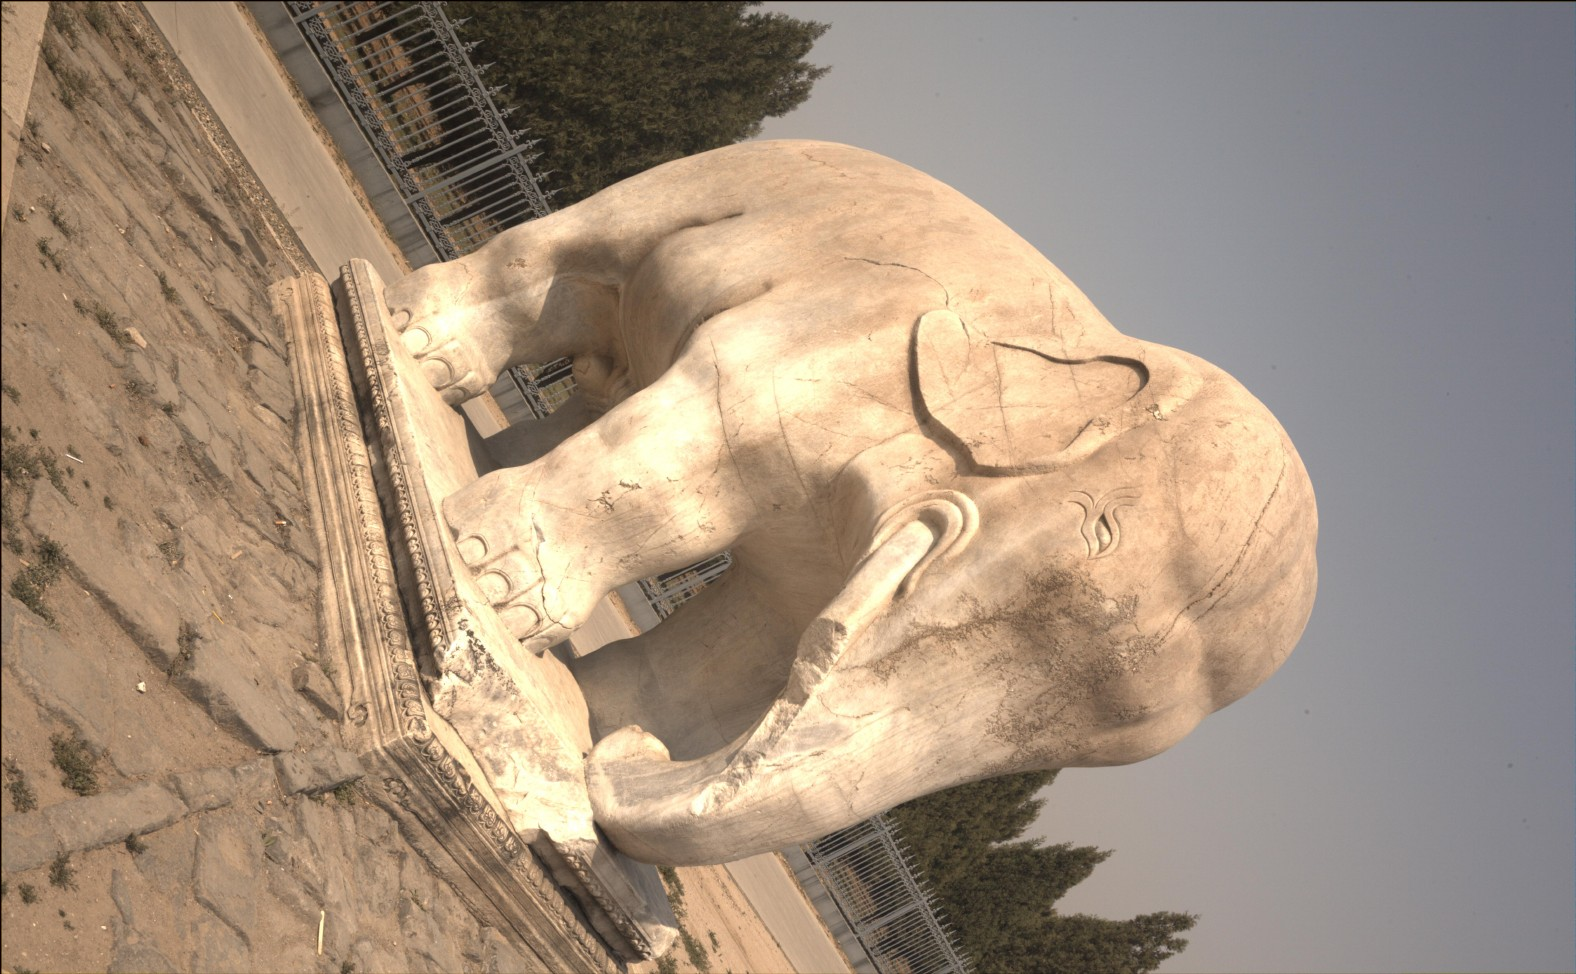
\includegraphics[width=80mm]{FIGS/SAMPLES/DoocDOC-Eleph-Photo.jpg} &
   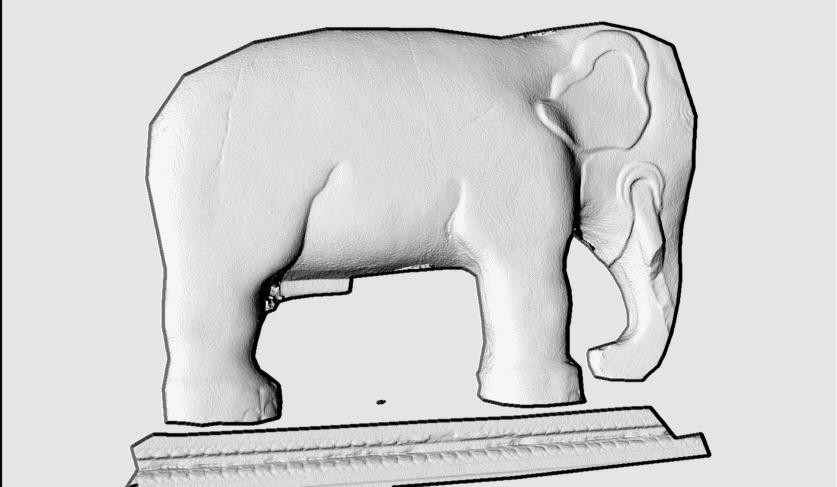
\includegraphics[width=80mm]{FIGS/SAMPLES/Doc-Elph-Shade.jpg}   \\ \hline  \hline
   \multicolumn{2}{||c||}{ 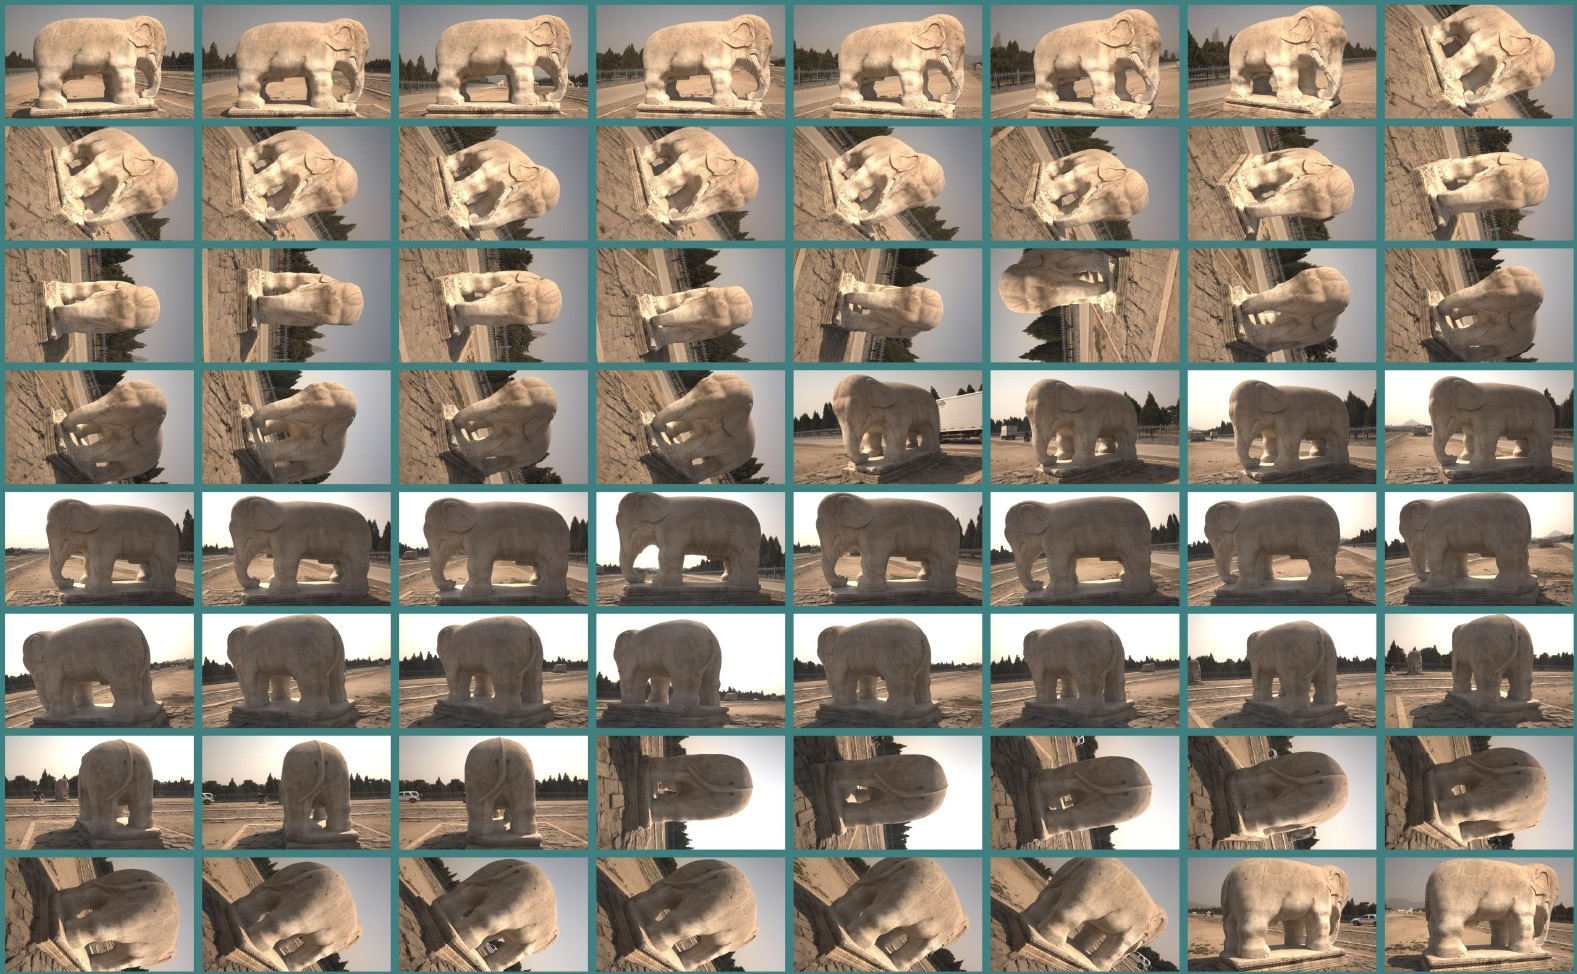
\includegraphics[width=150mm]{FIGS/SAMPLES/Doc-Pl-Eleph.jpg}} \\ \hline  \hline
   \multicolumn{2}{||c||}{ 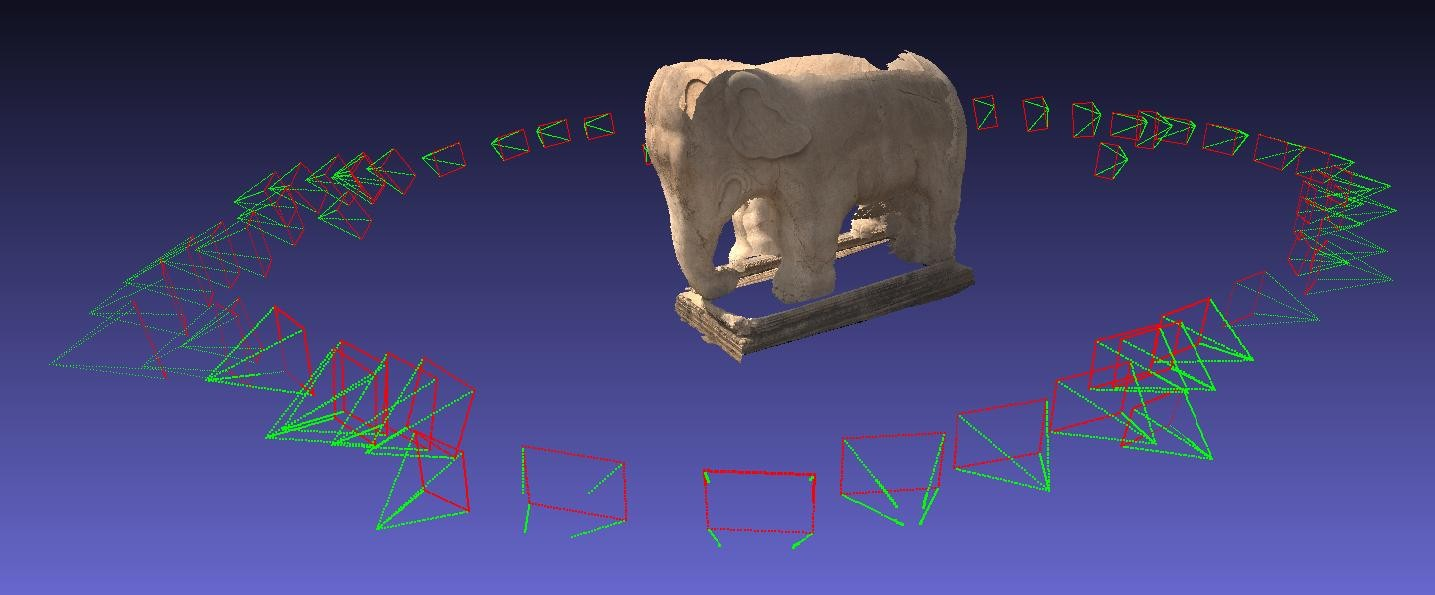
\includegraphics[width=150mm]{FIGS/SAMPLES/Doc-Eleph-3D.jpg}} \\ \hline  \hline
\end{tabular}
\caption{{\bf Statues:} elephant in Chian long temple, one of the 60 image, a shaded mode, a global view of the 60 image,
the $3$D model and the camera position}
\label{View:Eleph}
\end{figure}

\begin{figure}
\begin{tabular}{||c|c|c|c||}
   \hline \hline 
   \includegraphics[width=40mm]{FIGS/SAMPLES/P1-AB.JPG} &
   \includegraphics[width=40mm]{FIGS/SAMPLES/P1-Shade.jpg} &
   \includegraphics[width=40mm]{FIGS/SAMPLES/P2-A.JPG} &
   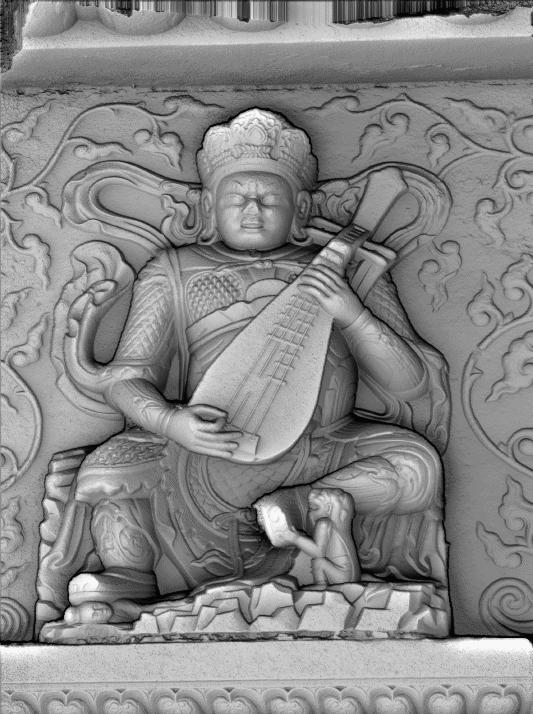
\includegraphics[width=40mm]{FIGS/SAMPLES/P2-Shade.jpg} \\
  \\ \hline  \hline
\end{tabular}
\caption{{\bf Statues:} Zhenjue temple}
\label{View:Eleph}
\end{figure}




\begin{figure}
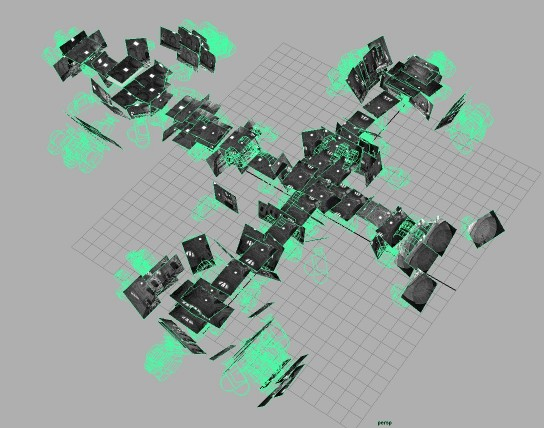
\includegraphics[width=70mm]{FIGS/SAMPLES/Aj2.jpg}
\includegraphics[width=100mm]{FIGS/SAMPLES/Aj1.jpg}
\caption{{\bf Indoor architecture: } Chapelle imperiale Ajacio, with 100 fish-eye images;
left position of camera, right 3D model}
\end{figure}



\begin{figure}
\includegraphics[width=160mm]{FIGS/SAMPLES/Pompei-Planche.jpg}
\includegraphics[width=160mm]{FIGS/SAMPLES/Pompei-Shade2.jpg}
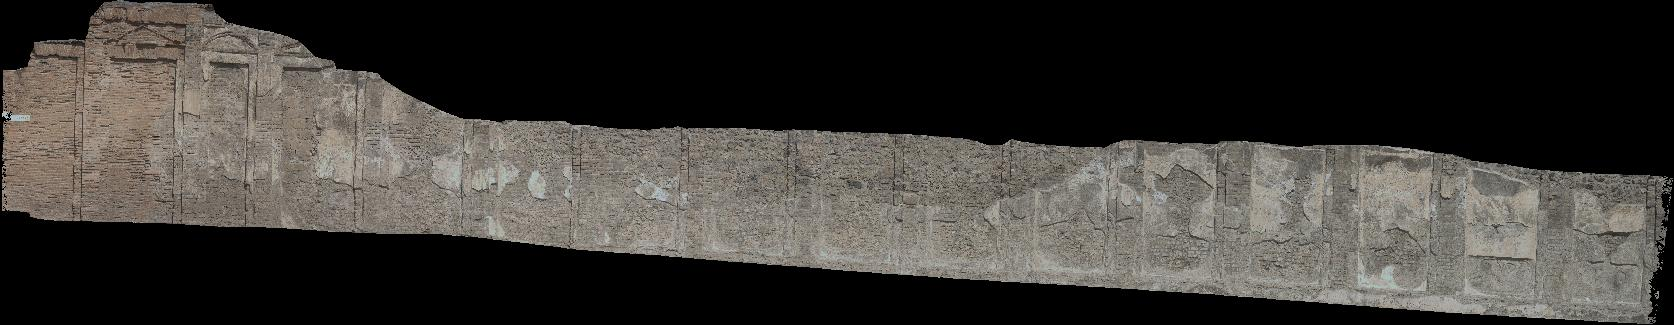
\includegraphics[width=160mm]{FIGS/SAMPLES/Pompei-Ortho1.jpg}
\caption{The set of images acquired on a wall in Pompei, a global
view of the 3D model of the wall and a global view of orthophoto}
\end{figure}

\begin{figure}
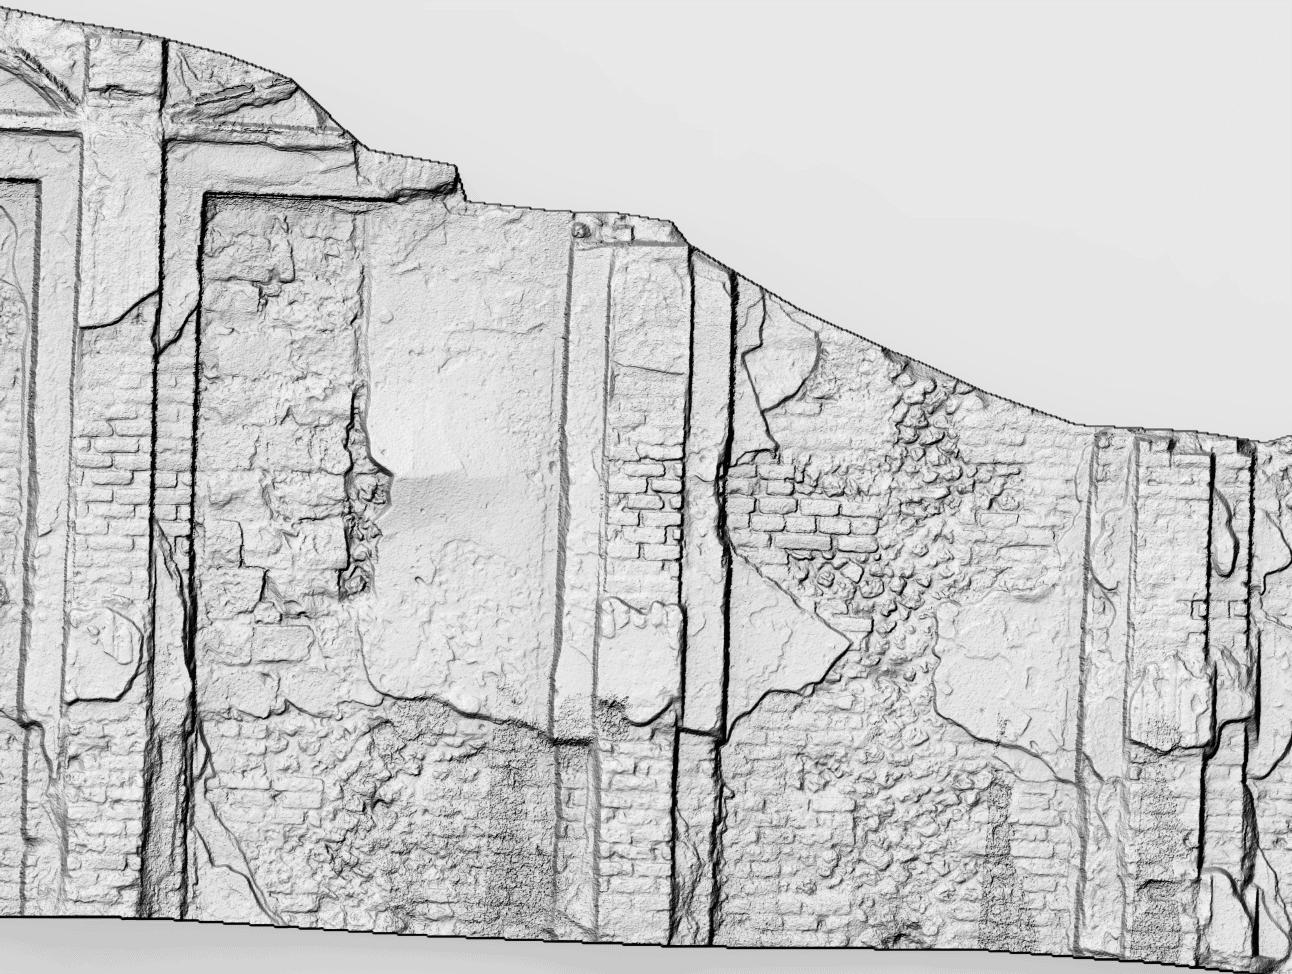
\includegraphics[width=70mm]{FIGS/SAMPLES/Pompei-Shade1.jpg}
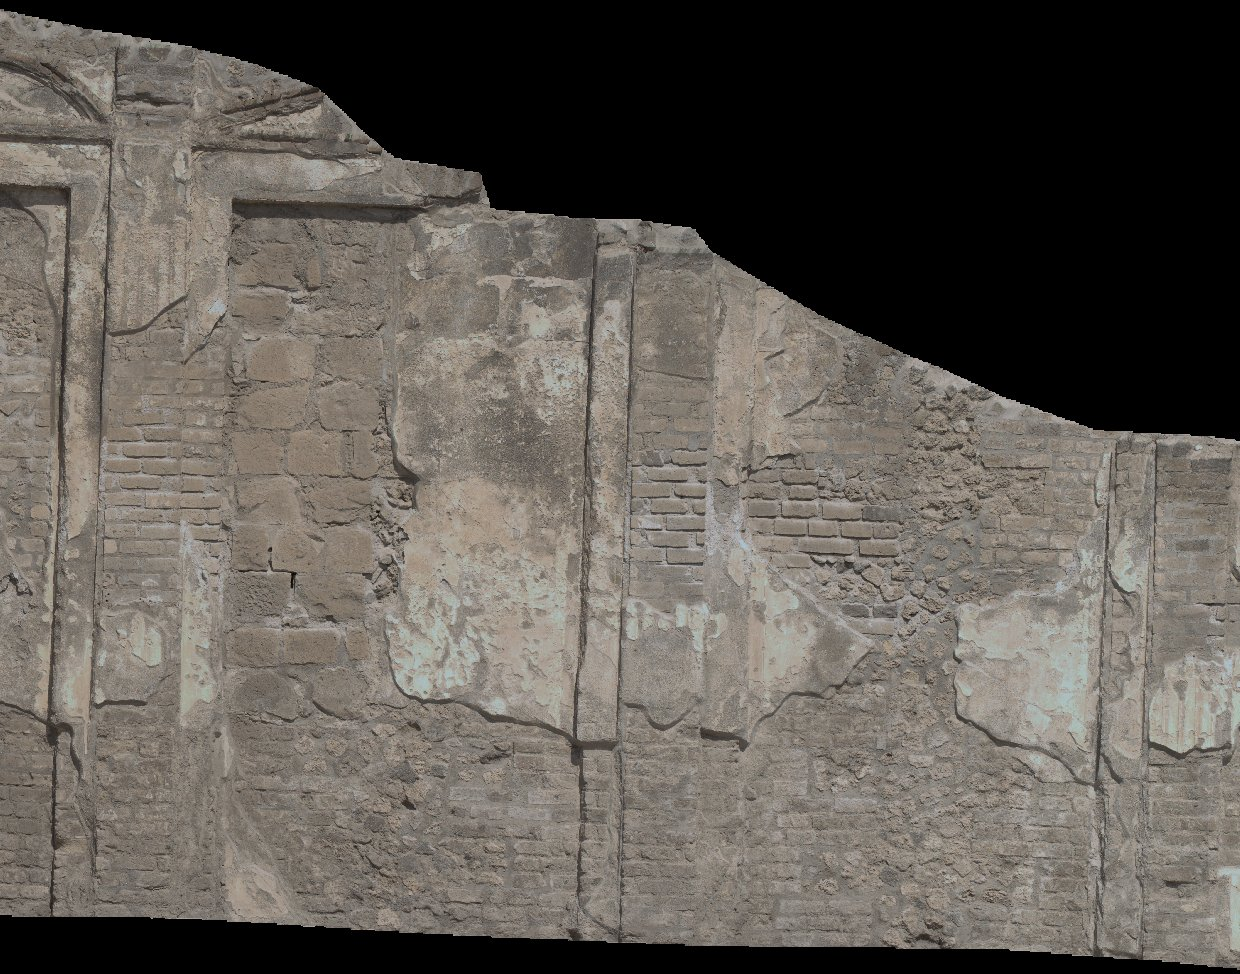
\includegraphics[width=70mm]{FIGS/SAMPLES/Pompei-Ortho2.jpg}
\caption{Detail on 3D model and otho photo in Pompei}
\end{figure}


\begin{figure}
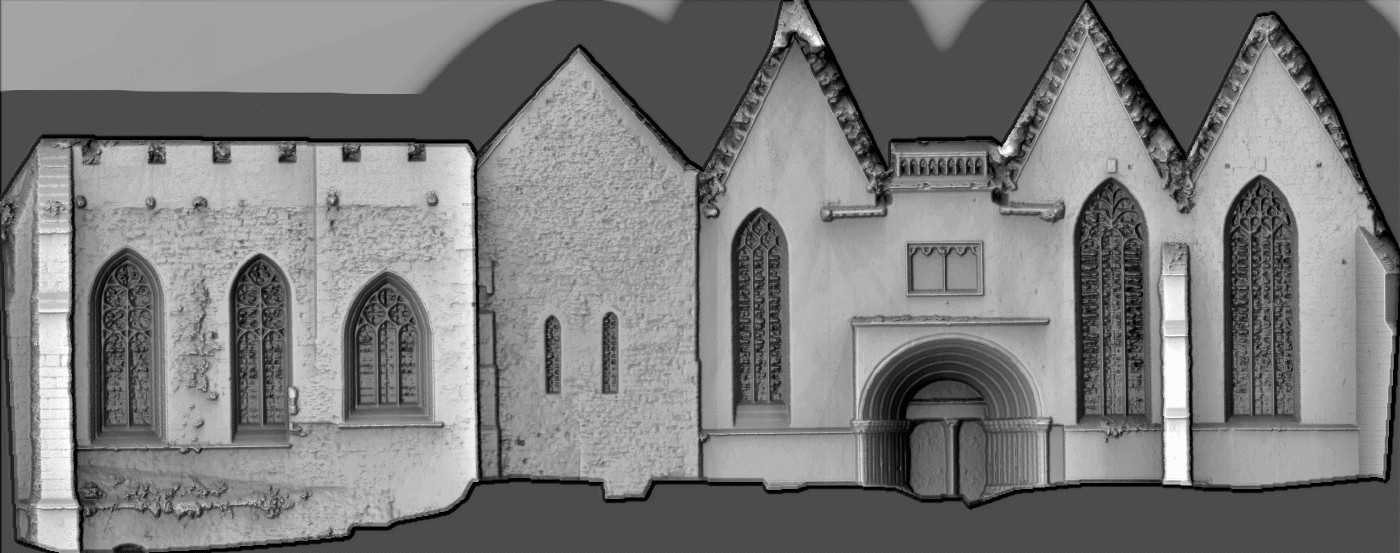
\includegraphics[width=150mm]{FIGS/SAMPLES/LambaleShade.jpg}
\includegraphics[width=150mm]{FIGS/SAMPLES/Lamballe-Ortho-Test-Redr.jpg}
\caption{3D model and otho photo on "Collégiale Notre Dame de la Garde (Lamballe)"}
\end{figure}




\begin{figure}
\includegraphics[width=90mm]{FIGS/SAMPLES/Louvre-Superp.jpg}
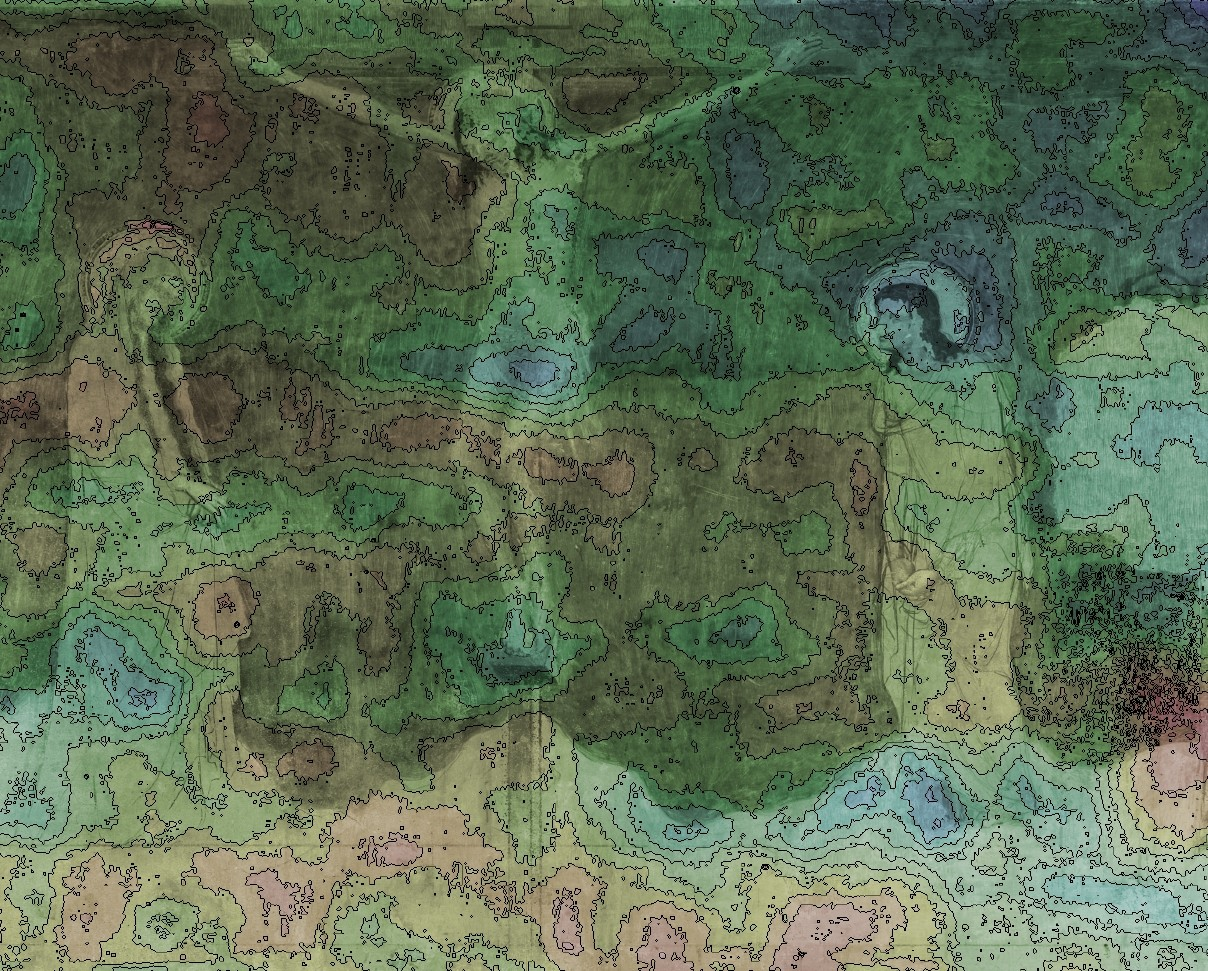
\includegraphics[width=90mm]{FIGS/SAMPLES/FresqVilAv.jpg}
\caption{{\bf Painting and Fresco: } CFine depth maps computation on painting and fresco,
images and in superposition level curves and hypsometry;
left image  , photo C2RMF/Jean Marsac; right fresque in Villeneuve
les Avignon, photo CICRP/Odile Guillon}
\end{figure}



\begin{figure}
\begin{tabular}{||c|c|c|c||}
   \hline \hline 
   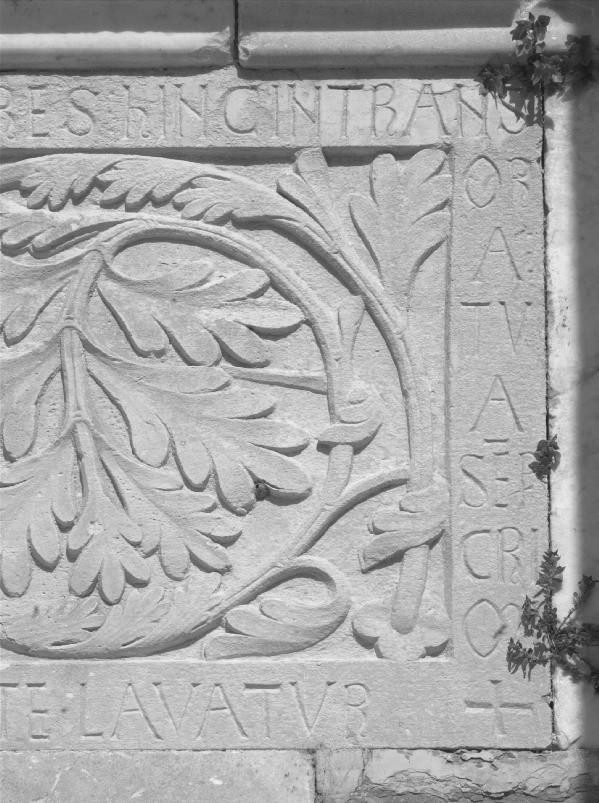
\includegraphics[width=40mm]{FIGS/SAMPLES/FRISE-IM1.jpg} &
   \includegraphics[width=40mm]{FIGS/SAMPLES/FRISE-IM2.jpg} &
   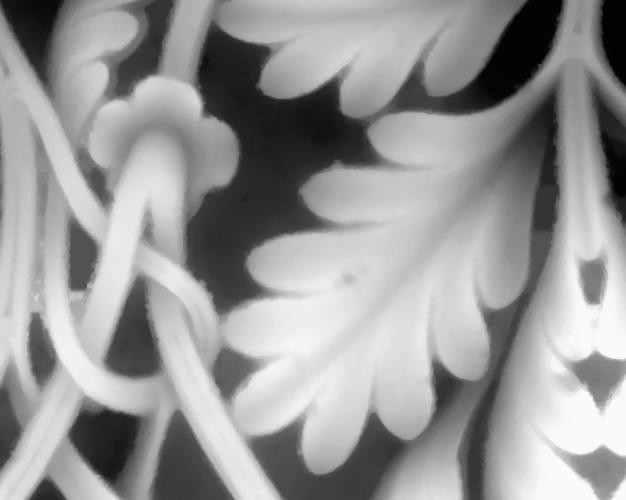
\includegraphics[width=40mm]{FIGS/SAMPLES/FRISE-Det1-F8Bits.jpg}&
   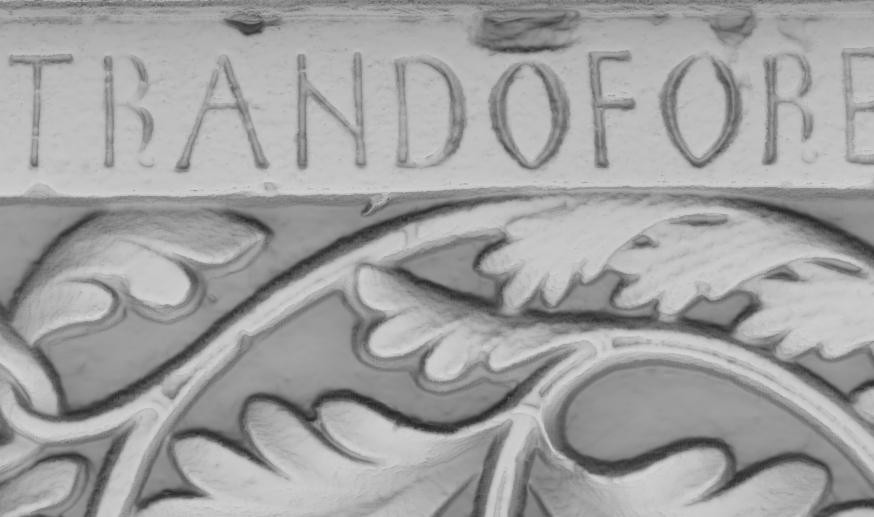
\includegraphics[width=40mm]{FIGS/SAMPLES/FRISE-Detail-ScaledShade.jpg} \\ \hline  \hline 
   \multicolumn{4}{|c|}{\vspace{2mm} 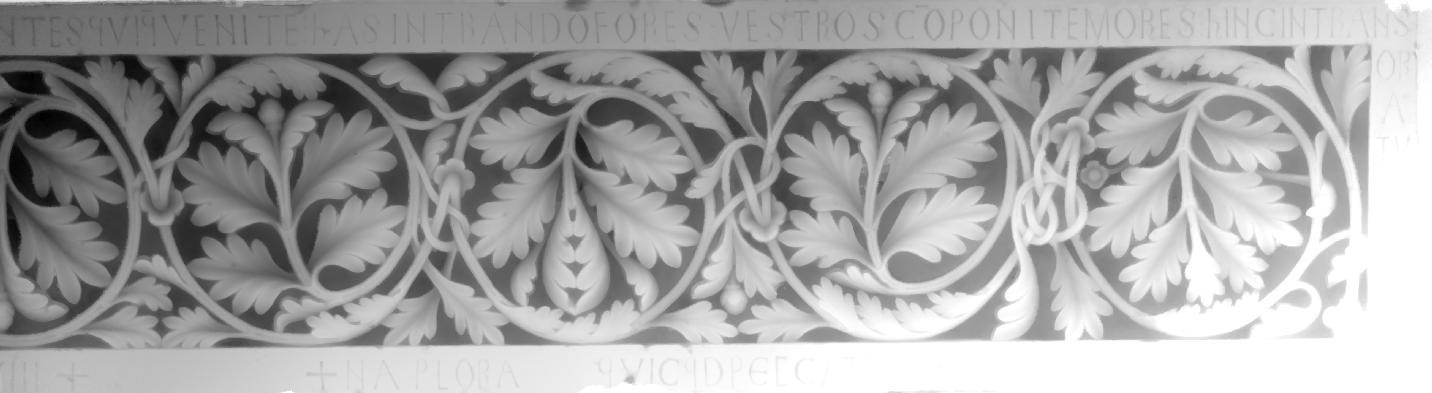
\includegraphics[width=160mm]{FIGS/SAMPLES/FriseDepthBits.jpg}} \\ \hline  \hline
   \multicolumn{4}{|c|}{\vspace{2mm} 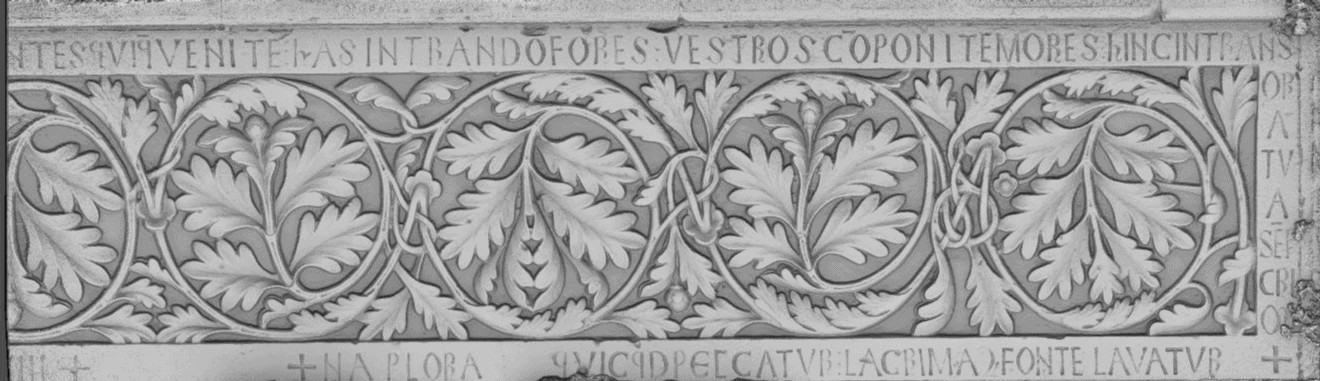
\includegraphics[width=160mm]{FIGS/SAMPLES/FrisScaledShade.jpg}} \\ \hline  \hline
\end{tabular}
\caption{{\bf Bas Relief} Frise in Villeneuves lez maguellone \dots}
\end{figure}


\begin{figure}
\begin{tabular}{||c|c|c||}
   \hline \hline 
   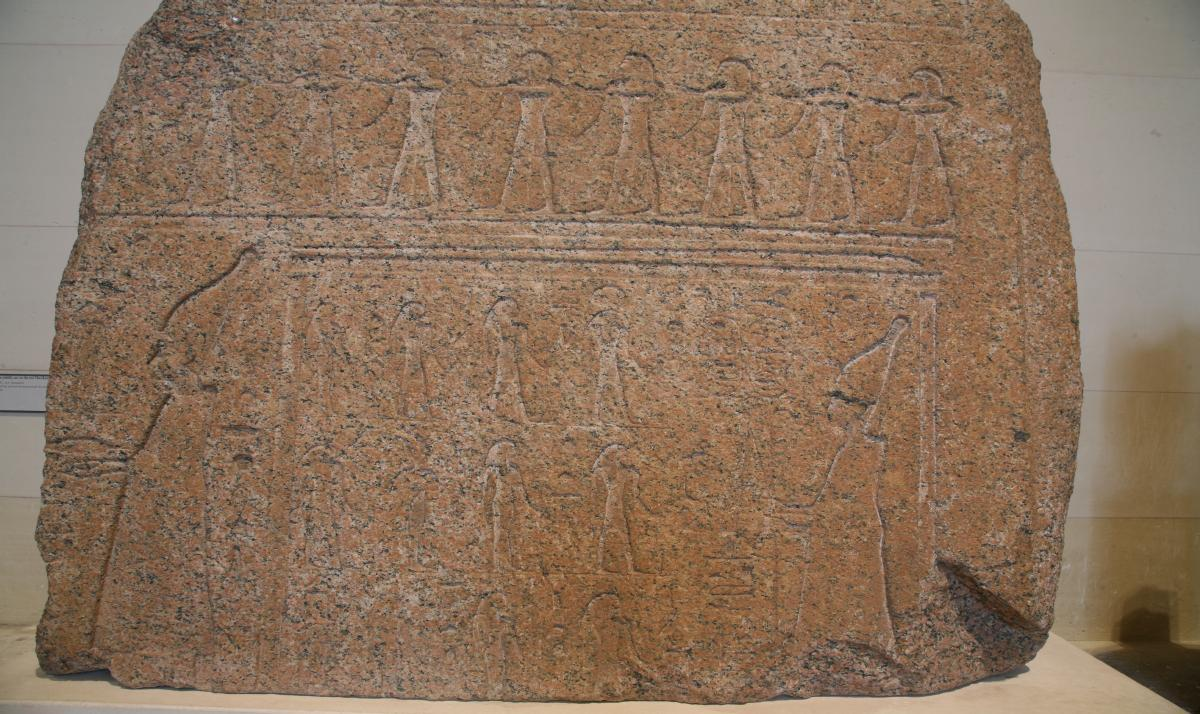
\includegraphics[width=60mm]{FIGS/SAMPLES/Hiero1_2908.JPG} &
   \includegraphics[width=60mm]{FIGS/SAMPLES/Hiero2_2908.JPG} &
   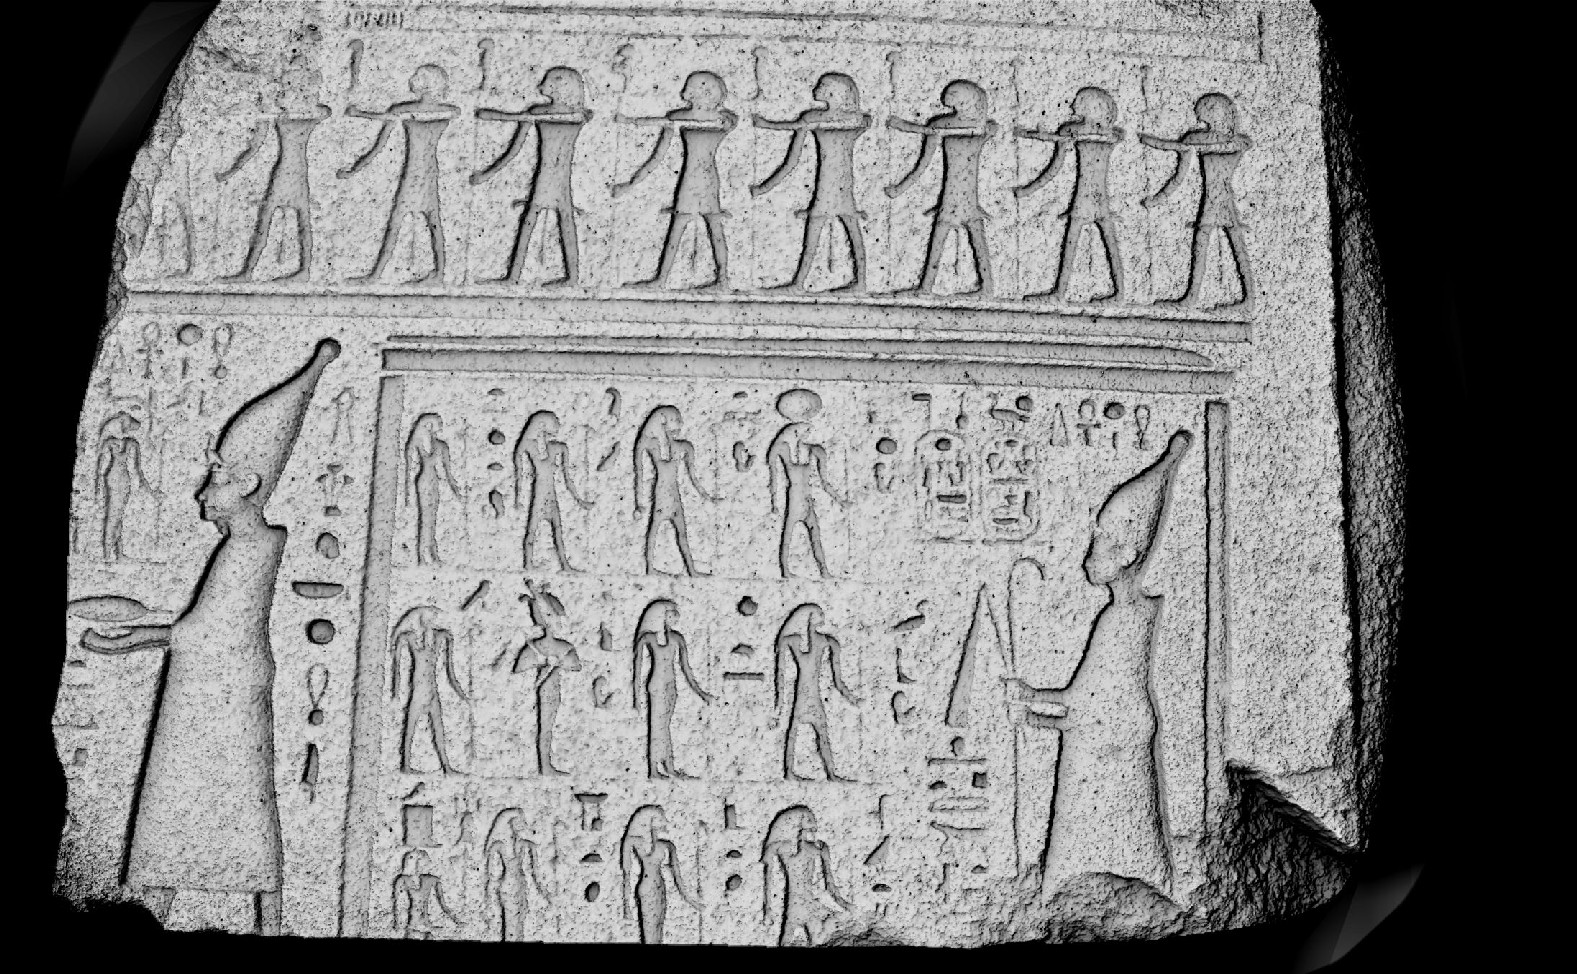
\includegraphics[width=60mm]{FIGS/SAMPLES/Hiero3_2908.JPG} \\ \hline  \hline 
\end{tabular}
\caption{{\bf Bas Relief} Stele in Louvre , image and 3D model rendered in shading and depth map \dots}
\end{figure}



\begin{figure}
\begin{tabular}{||c|c||}
   \hline \hline 
   \includegraphics[width=80mm]{FIGS/SAMPLES/ROUFF-IM.JPG}&
   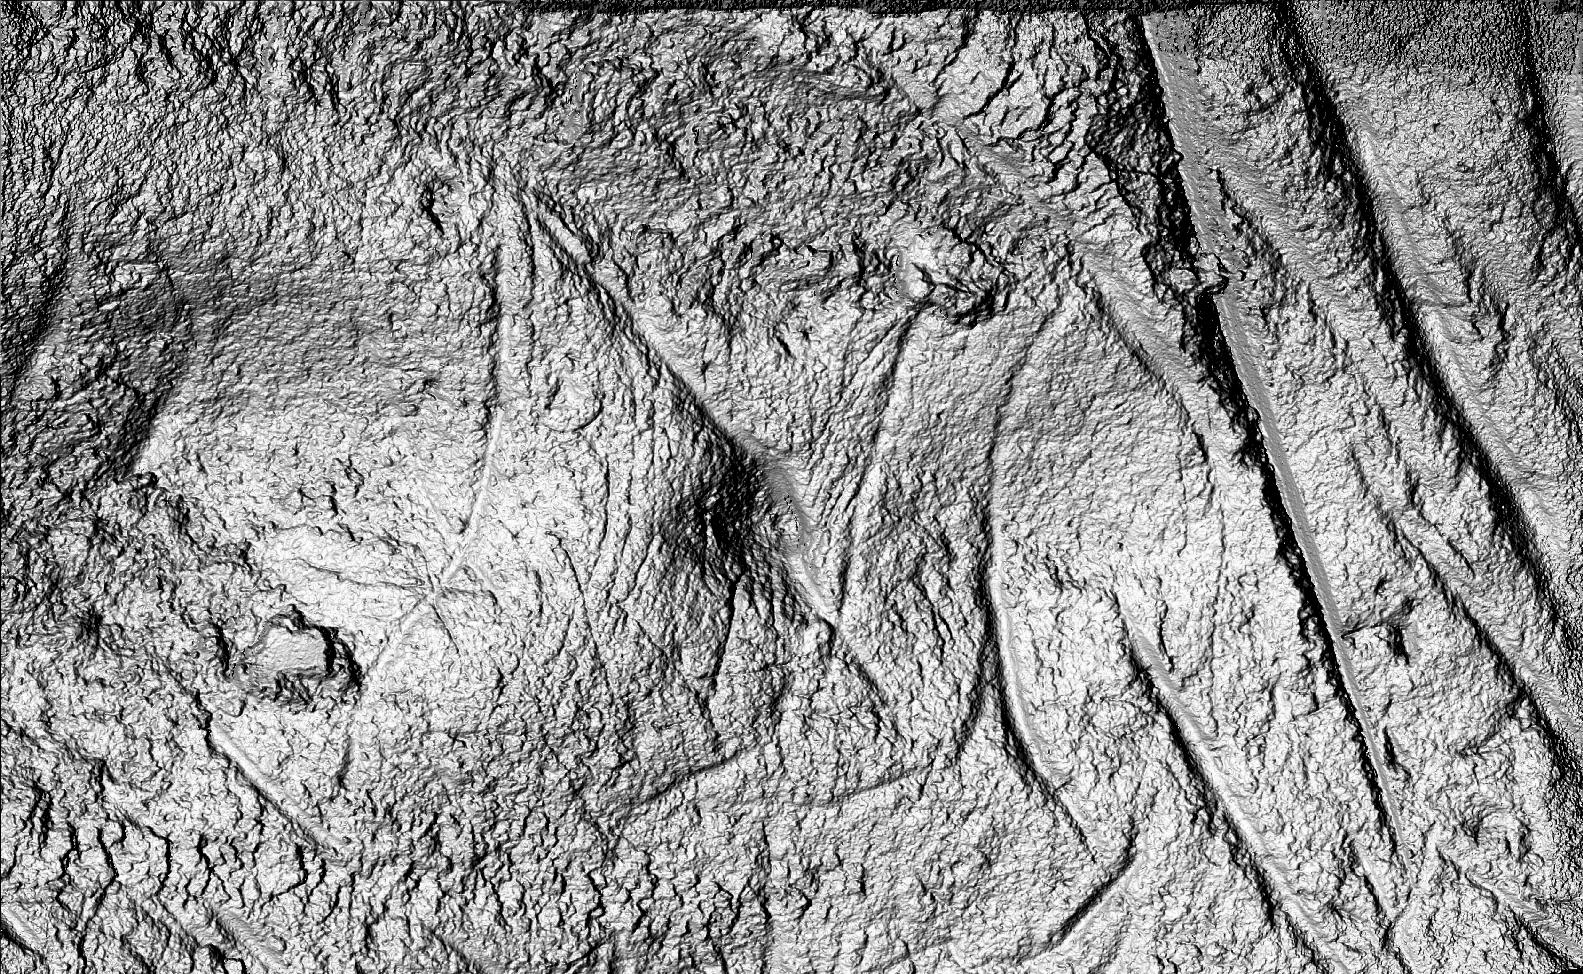
\includegraphics[width=80mm]{FIGS/SAMPLES/ROUFF-SHADE.jpg} \\ \hline  \hline 
\end{tabular}
\caption{{\tt Macro photography} in rouffignac cave, at $\frac{1}{20}$ mm resolution : image and shading of 3D model \dots}
\end{figure}


\begin{figure}
\begin{tabular}{||c|c||}
   \hline \hline 
   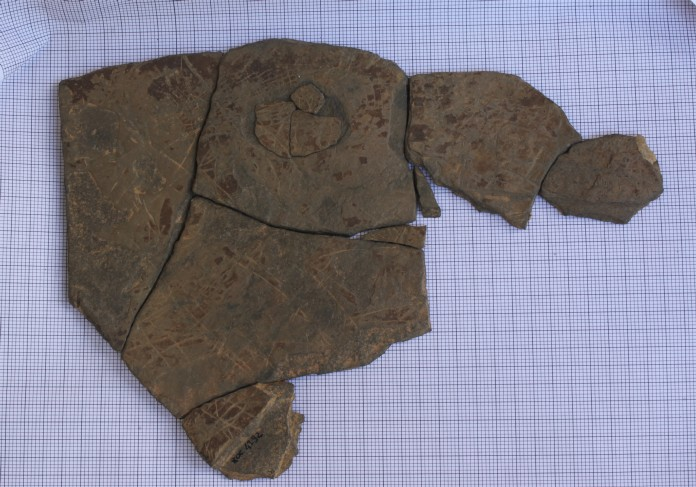
\includegraphics[width=80mm]{FIGS/SAMPLES/Doc-Pijo1.jpg}&
   \includegraphics[width=80mm]{FIGS/SAMPLES/Doc-Pijo2.jpg} \\ \hline  \hline 
    \multicolumn{2}{|c|}{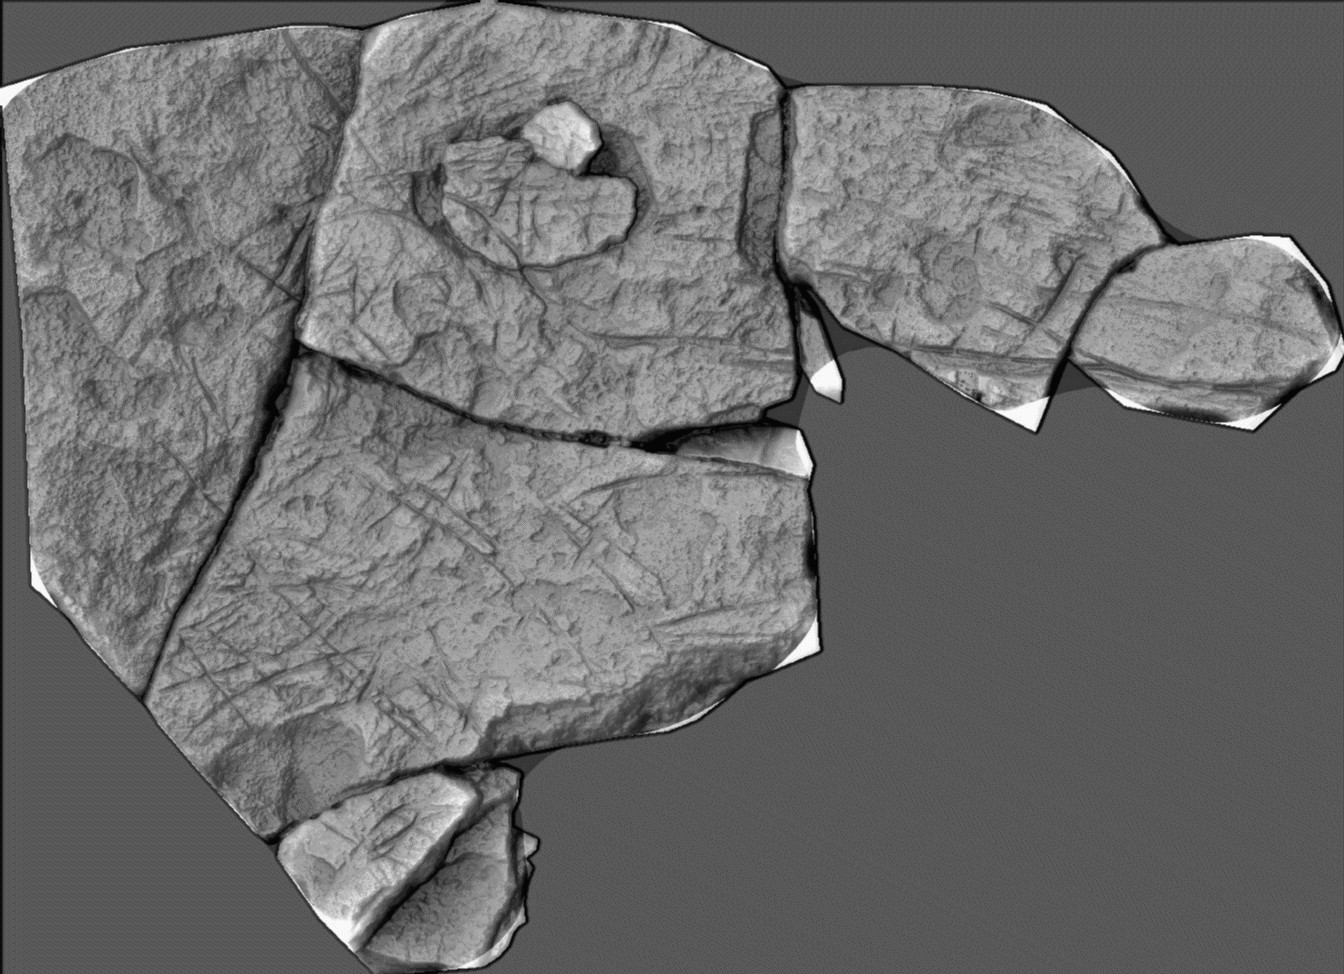
\includegraphics[width=150mm]{FIGS/SAMPLES/Doc-Pijo3.jpg}}  \\ \hline  \hline
\end{tabular}
\caption{{\tt Macro photography} plaquette of cave Mayenne science \dots}
\end{figure}











\begin{figure}
\includegraphics[width=90mm]{FIGS/SAMPLES/DGPF_8Bits.jpg}
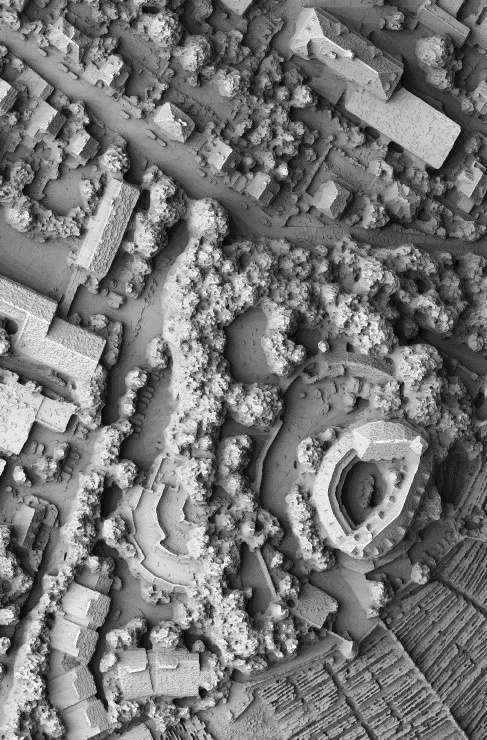
\includegraphics[width=90mm]{FIGS/SAMPLES/DGF-SHADE.jpg}
\caption{Digital elevation model on semi urban area, 8cm resolution, DGPF data set, for
Euro-SDR benchmarkin on image matching}
\end{figure}

\begin{figure}
\includegraphics[width=180 mm]{FIGS/SAMPLES/DGPF-GLOB.jpg}
\caption{A more global view of DEM on DGPF data set}
\end{figure}




\begin{figure}
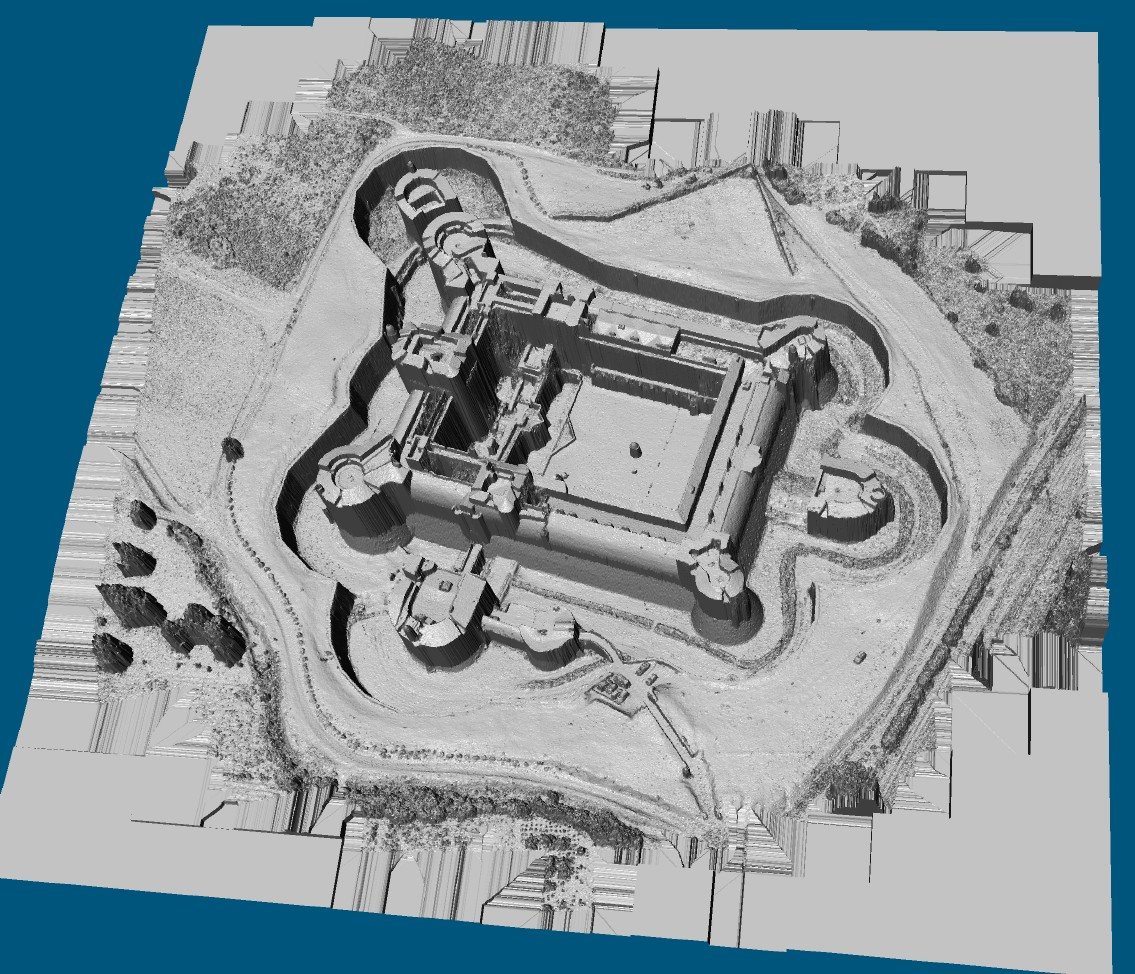
\includegraphics[width=90 mm]{FIGS/SAMPLES/SlsMNE_1_25.jpg}
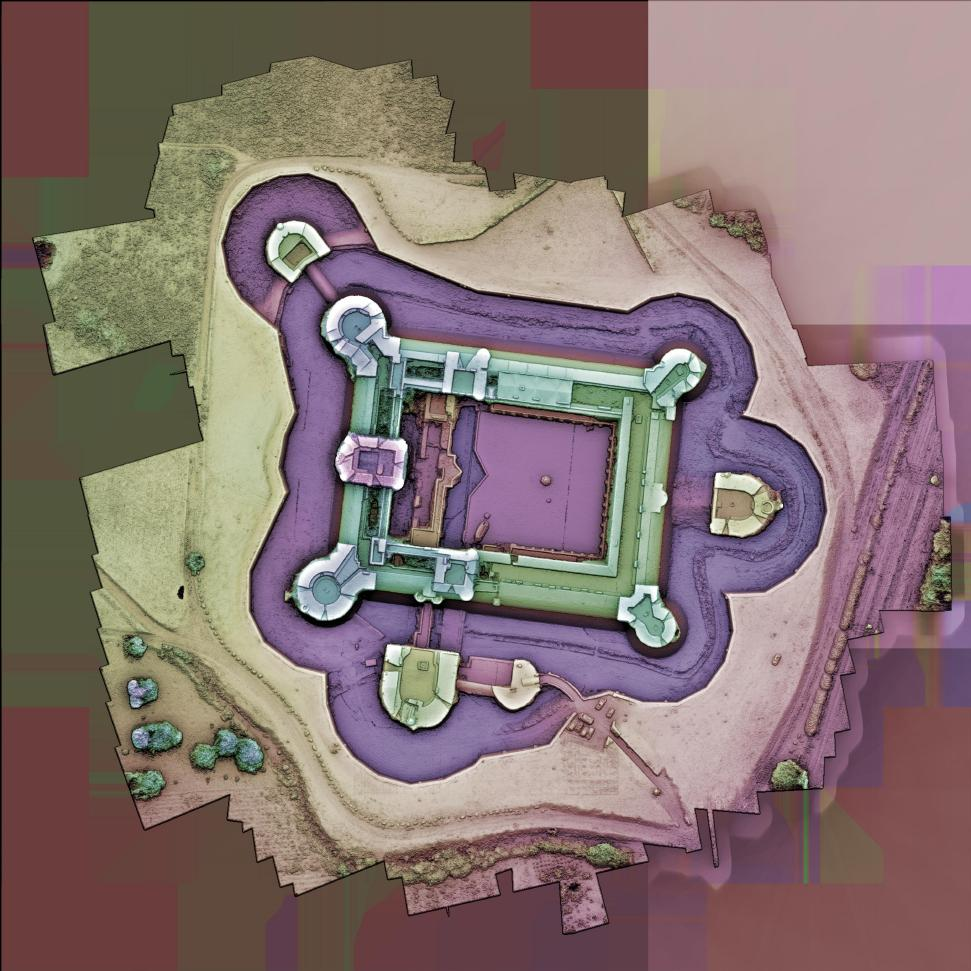
\includegraphics[width=90 mm]{FIGS/SAMPLES/Salse2.jpg}
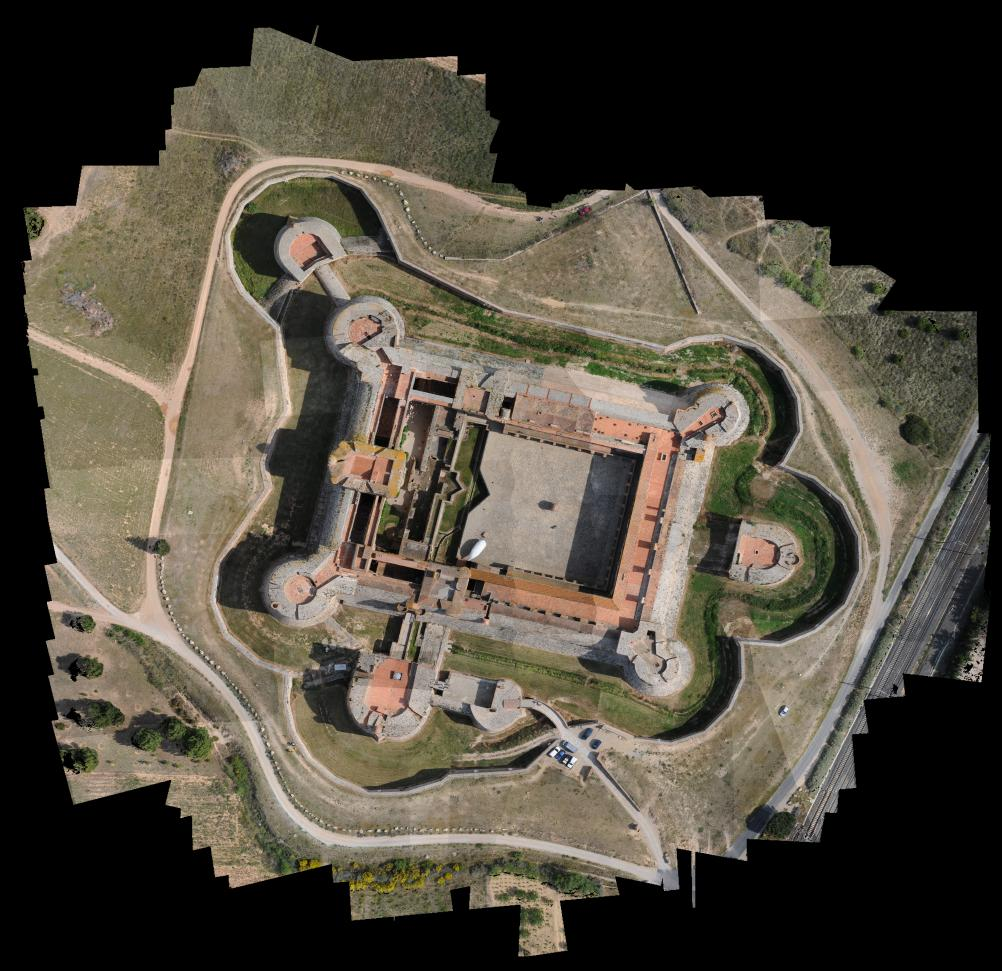
\includegraphics[width=90 mm]{FIGS/SAMPLES/Ortho-Test-Redr.jpg}
\caption{Forteresse de Salses, photo acquired by drone survey, in collaboration
with Map-CNRS; oblique view of 3D model, hypsometry and shading, ortho photography
Euro-SDR benchmarkin on image matching}
\end{figure}



